%!TEX root = ../../thesis.tex

\section{Word properties}
\label{chapter:limitations:wordlproperties}


\question{How the world properties (symmetries, size, \ldots) affect the learning properties?}

As discussed in chapter~\ref{chapter:lfui:symmetries}, the properties of the world can affect the learning performances. For example some worlds have symmetric properties which makes some tasks impossible to differentiate.

In this section, we compare how various planning method perform on our two different worlds, namely the pick and place scenario and the grid world. We will investigate a random strategy, several $\epsilon$-greedy (where the agent follows the best strategy or select an action randomly $\epsilon$ of the times), a strategy based on the task uncertainty (where we do not take the signal to meaning mapping uncertainty in to account), and our uncertainty based method described in chapter\ref{chapter:planning}. We will see that the size and the optimal policies properties of each world impacts the performances of some planning methods.

\subsection{Hypothesis and world properties}

Our hypothesis is that differences in size and optimal policies properties of each world will impacts the performances of some planning method considered, especially the random method which was performing quite well in our previous examples of chapters~\ref{chapter:planning}~and~\ref{chapter:bci}.

In the coming analysis we will consider three different world, a 5 by 5 grid world, a 25 by 25 grid world and our pick and place world of chapter~\ref{chapter:lfui}. In the following we present the main differences between those worlds.

First testing our planning method on a 5x5 and 25x25 allow to test how the size of the world influence the performance of each of the method and verify that our uncertainty measure is robust to such change. The main hypothesis is that the random action selection method will not scale well to this change in dimensionality. In a 5x5 grid, random actions allow to cover the space quite uniformly in 100 time steps, however in a 25x25 the robot will not succeed in exploring all the state and is therefore unlikely to visit useful states at every experiments.

We choose to use a 25x25 grid because the resulting number of state (625) is similar to the number of state of our pick and place scenario (624), which allow to remove the size effects when comparing those two scenarios. By comparing the grid world and the pick and place scenario, we aim at investing how the maze like properties of the pick and place word compares with the less strict properties of the grid world. For the pick and place scenario, to reach the correct cube configuration the robot must achieve a very specific sequence of action in the correct order. Like for going out of a maze, only one correct path can be followed. However for the grid world, a multitude of path can be chosen. 

This can be measure by the amount of overlap between the optimal policies associated to two ``close'' task. For the pick and place scenario, if the signal to meaning mapping were known, to differentiate between two cube configuration that are close together, the agent must go towards those configuration to be able to discard one or an other task. For example, in our illustration of Figure~\ref{fig:lfui:pickplacesequence}, to differentiate between the two first state, one as to reach one of those two states to tell the identify the correct one. Indeed, their corresponding optimal policies are similar for every state except their two final states, i.e. both tasks share the same policies for 622 states our of 624. However for the grid world scenario, if the signal to meaning mapping were known, one could differentiate between the top right state and the state directly on the left of that top right state by simply performing a left action on the bottom right state. And this whatever the size of the grid. The optimal policies of those two task differs for all states along the two columns on the left of the grid, i.e. both tasks share the same policies for only 575 states our of 625 in our 25x25 grid world.

\subsection{Method}

We used the same condition as used in chapter~\ref{chapter:planning}, where the teacher is providing instruction following the feedback frame and using two dimensional signals of very good quality (i.e. between 90 and 100 percent of classification rate).

We simulated 50 runs for each planning method and each world considered. There where 10 steps of initialization before the agent starts computing the first likelihood. During the first 10 steps, the agent where actiong randmly for all methods.

\subsection{Results}

In this subsection, we will analyze the Figure~\ref{fig:wordlpropertiestimefirst} which displays the number of iterations needed for our agent to reach a first task depending on the planning method and the worlds. We will first consider the difference between the 5x5 grid world and the 25x25 grid world, and then compare the grid world and the pick and place scenario.

\begin{figure}[!ht]
\centering
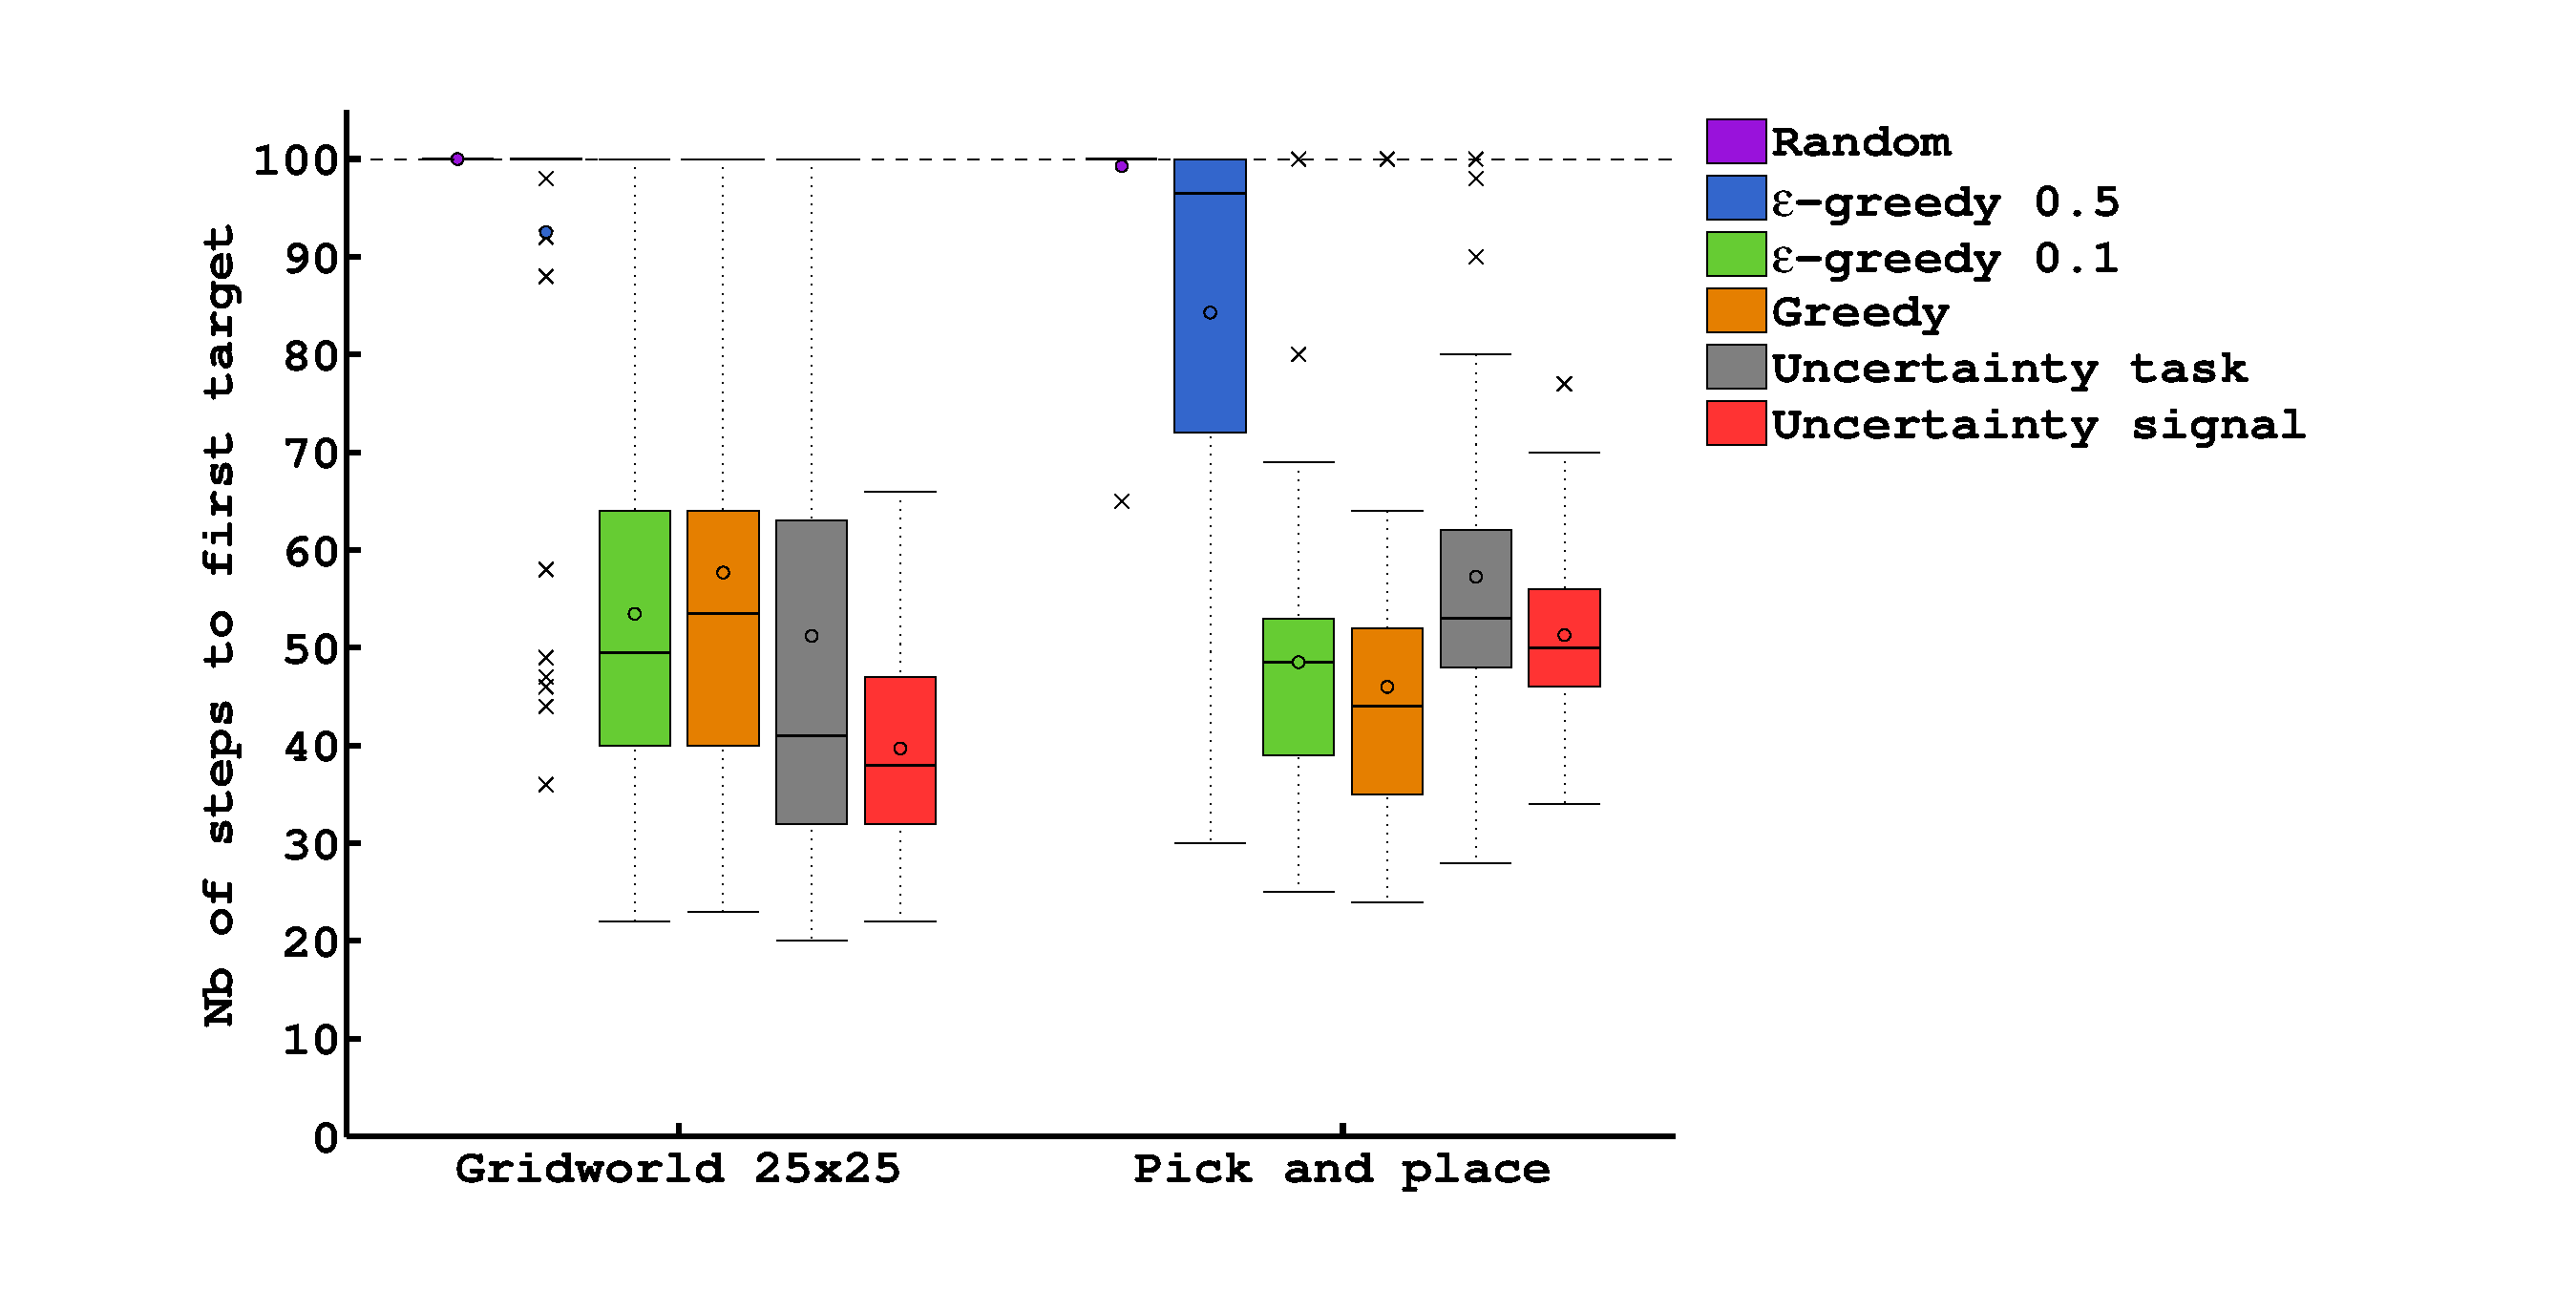
\includegraphics[width=\legendsidesize\columnwidth]{\imgpath/world_properties/firstreach.eps}
\caption{Number of steps to reach first target state with confidence. Comparing different action selection methods and different worlds. As soon as the dimensionality increase, selecting action randomly can not identify any task in 100 iterations. Our signal uncertainty based method, is the most efficient at reaching the first task in the grid world but seems outperformed by a simple greedy approach in our pick and place scenario.}
\label{fig:wordlpropertiestimefirst}
\end{figure}

Before analyzing the results, there is several aspects that are important have in mind. First, Figure~\ref{fig:wordlpropertiestimefirst} displays the number of step needed to reach the target state while being confident this state is the correct one. The agent can become confident one task is the correct one while being in a state far from the goal state associated to that task. When the agent is confident about one task, it acts greedily according the optimal policies associated to that task. This fact will play an important role in our analysis of the pick and place results and on the following discussion.

Also, when a method was not able to reach a task with confidence in 100 steps we considered a value of 100 for our plots. This is very optimistic for the corresponding methods, for example the random method is likely to need more than 100 steps in our larger worlds. We report the number of runs than reached a first target in less than 100 iterations in Table~\ref{tab:wordlpropertiesnreach}, which indicates that only our uncertainty based method was able to identify a task in less than 100 steps for every run. 

\begin{table}[!ht]
\centering
\rowcolors{2}{gray!25}{white}
\begin{tabular}{c c c c}
    Planning methods & Gridworld 5x5 & Gridworld 25x25 &  Pick and place \\ \hline
    Random & 47 & 0 & 1 \\ 
    $\epsilon$-greedy 0.5 & 50 & 13 & 27 \\
    $\epsilon$-greedy 0.1 & 46 & 48 & 48 \\
    Greedy & 41 & 43 & 47 \\
    Uncertainty task & 45 & 42 & 48 \\
    Uncertainty signal & 50 & 50 & 50 \\
\end{tabular}
\caption{Number of experiments that reached at least one target in 100 steps.}
\label{tab:wordlpropertiesnreach}
\end{table}


Finally, our plots include correctly and wrongly identified first targets, however only a handful of task where incorrectly identified. We report only 12 erroneous first task estimations across all 900 runs of our experiments and conditions. For the 5x5 grid world, 1 error for the Random method, 1 for Uncertainty task and 1 for Uncertainty signal. For the 25x25 grid world, 1 error for the Greedy method. For the pick and place scenario, 1 for $\epsilon$-greedy 0.5, 2 for $\epsilon$-greedy 0.1, 2 for Greedy, 1 for Uncertainty task and 2 for Uncertainty signal.


\paragraph{World size effects}

As expected the random selection method fails at identifying a task when the state space grows. The first obvious observation is that all method requires more iteration to reach a first task when the size of the world increases. In a 5x5 grid world, a random strategy allows to visit a good percentage of the states which ensure the agent as collected useful evidence. However, a bigger world, it is important to target specific state. Interestingly, going toward the best estimate or using the uncertainty on the task only performs quite well, however only our uncertainty based method identified 50 times out of 50 the task in 100 steps.

When comparing with the results of chapter~\ref{chapter:planning} Figure~\ref{fig:artificialplanning}, the greedy method is here way better. The only difference lies in the dimensionality of the dataset. We note that in the experiment of this section, the agent start by 10 random movement before starting updating likelihood, and as the data are 2 dimensional and of high qualities, it is rather easy to have a reasonable estimate of each classifiers. However in the experiments  chapter~\ref{chapter:planning} Figure~\ref{fig:artificialplanning}, the agent used 30 dimensional data and performed 42 steps of initialization, which means there were less point per class than of dimension which is probably the explanation of the difference observed. The effect of the dimensionality and quality of the datasets remains to be investigated in more details.

\paragraph{Maze properties effects}

When comparing the performance on the grid world versus the pick and place world on Figure~\ref{fig:wordlpropertiestimefirst}, we observe that our uncertainty based planning method is no more the most efficient method in the pick place word. And that a very simple method such as acting greedy according to the current best task estimates performs better. We also note that the random method is unable to identify a task in less than 100 steps. This result is in line with the results form chapter~\ref{chapter:lfui} Figure~\ref{fig:selectionMethod} (left), where after 100 steps most of the task where identified after 100 steps using a Greedy planning method. However, for the random action selection method, the confidence level was still far out of reach after 100 steps.

The time to reach a target with confidence is in the end what will matter for the potential users of such a system. However none of the planning method presented above are taking this objective into account. Obviously the random or greedy methods are not following any specific goal, while the uncertainty based method only tries to reduce the uncertainty about the task but not to solve that task. That is why we switch to a pure exploitation of the task once the confidence level is reached.

Therefore it may be more relevant to look at the time needed to reach the confidence level for the first task, which is displayed in Figure~\ref{fig:wordlpropertiesconfidencefirst}. We note that our uncertainty method is in act faster at identifying the task that the greedy method seems to find more far away from the goal at that time.

\begin{figure}[!ht]
\centering
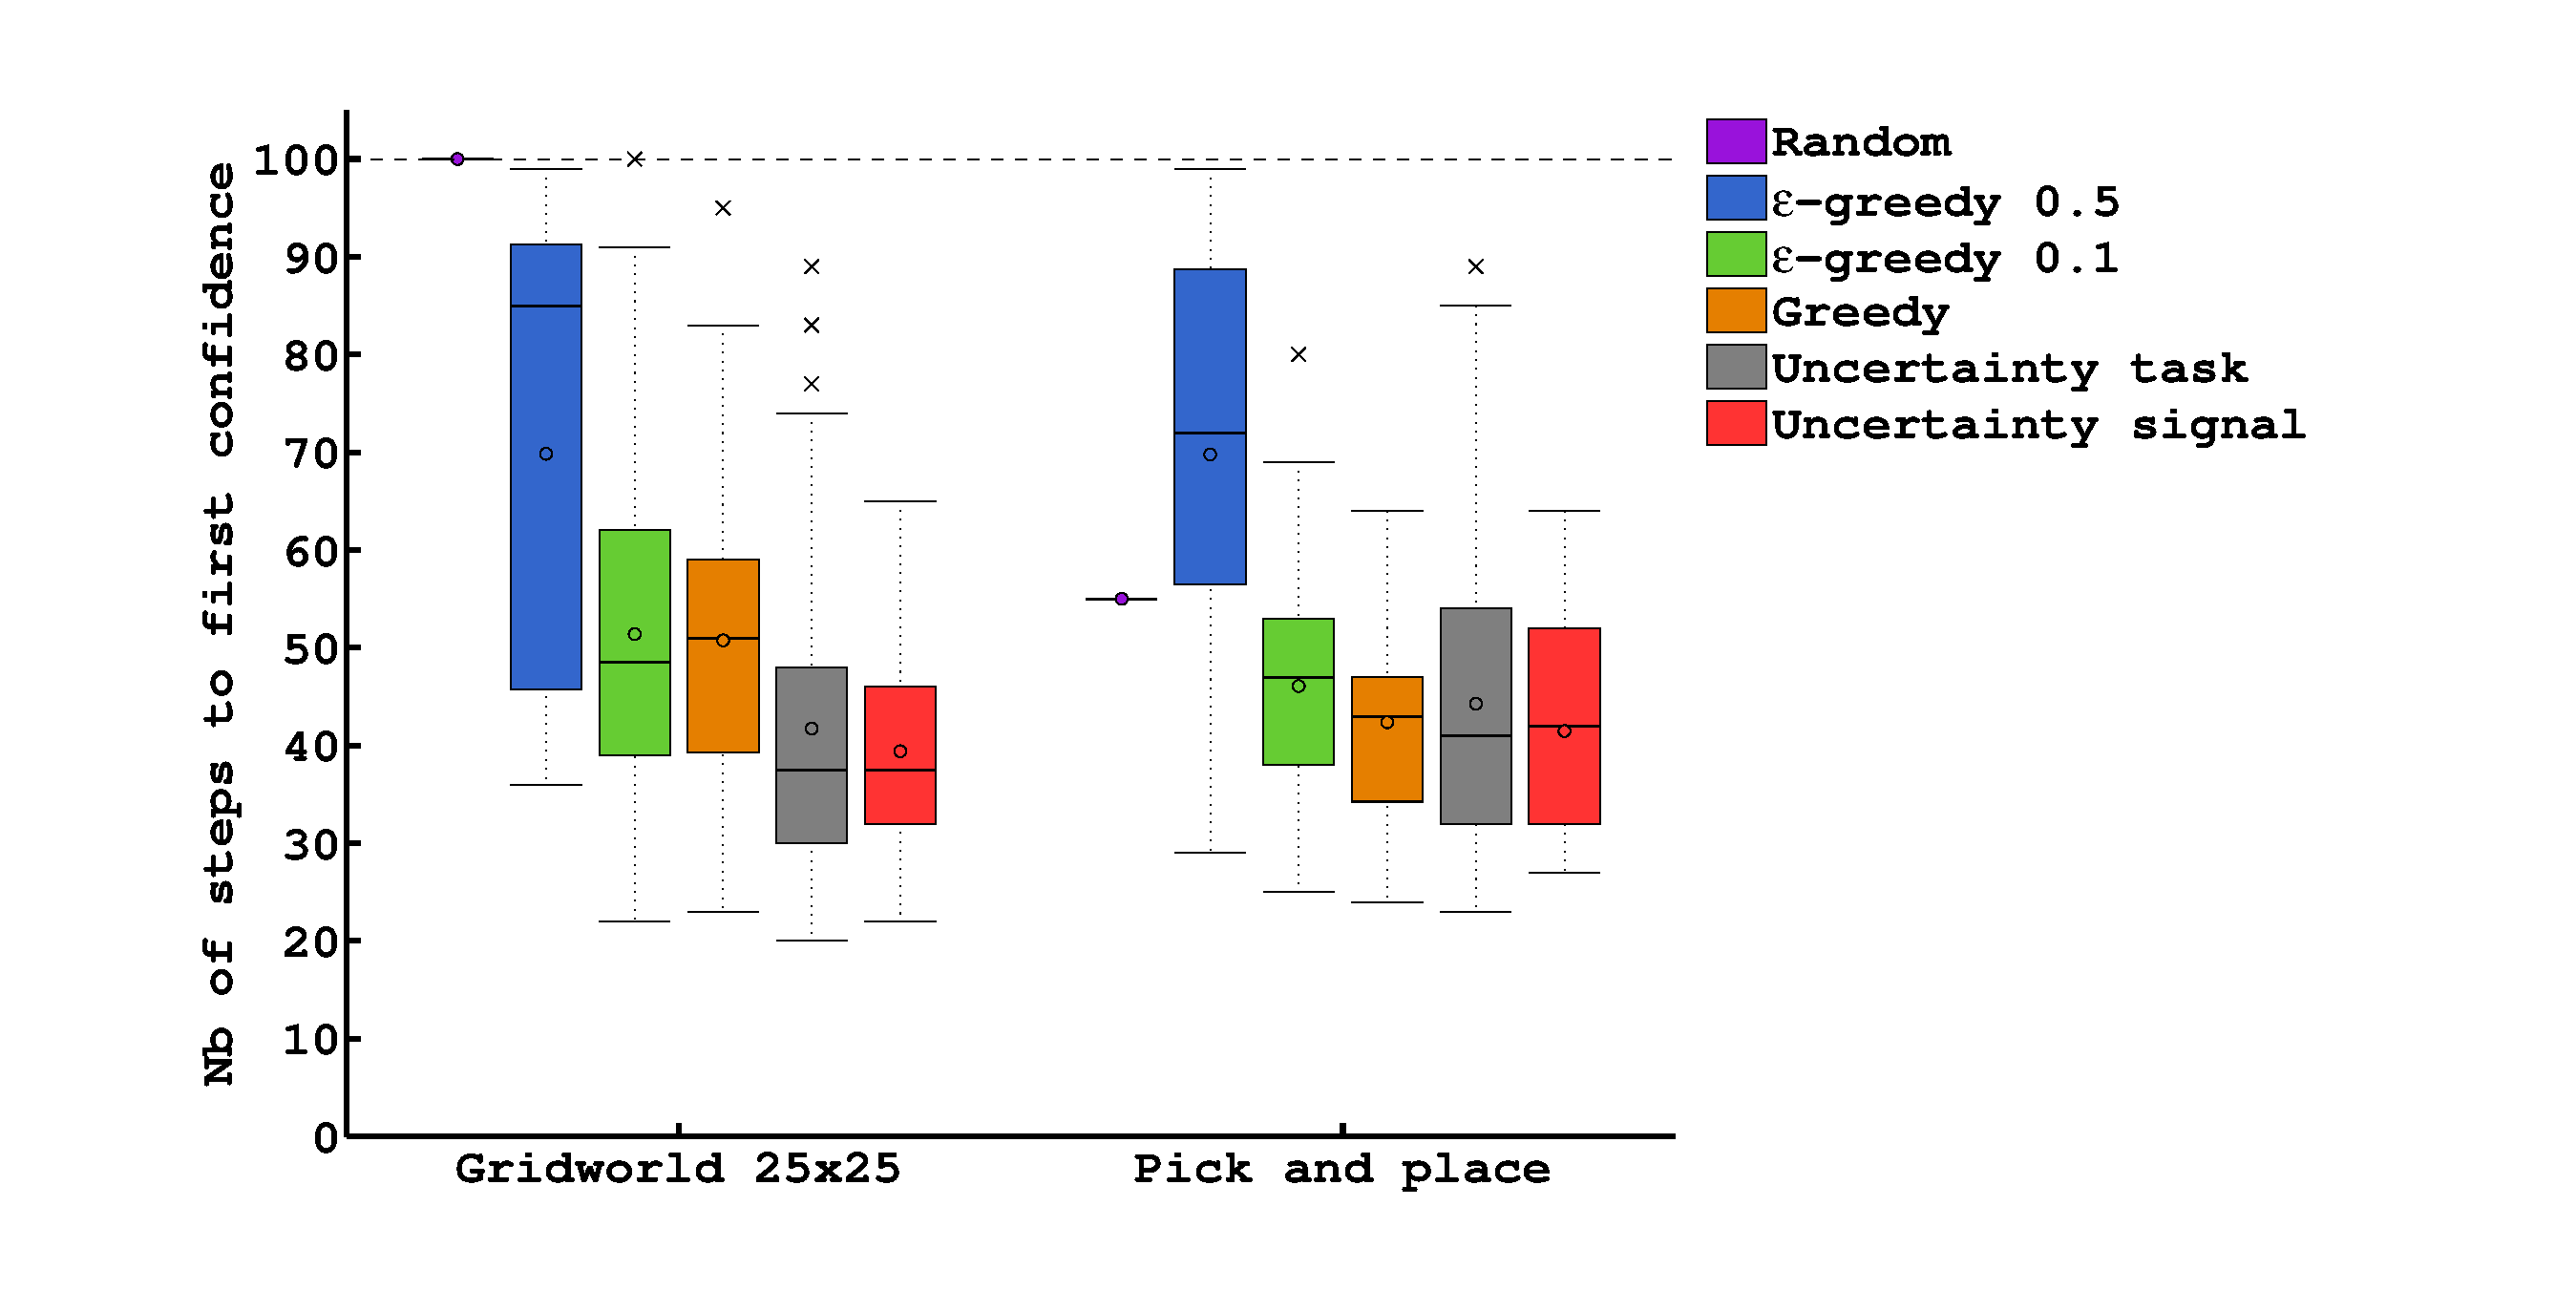
\includegraphics[width=\legendsidesize\columnwidth]{\imgpath/world_properties/firstconfident.eps}
\caption{Number of steps to reach confidence level for the first target.}
\label{fig:wordlpropertiesconfidencefirst}
\end{figure} 

Figure~\ref{fig:wordlpropertiestargetdist} shows the number of action needed for the agent to reach the goal state once the task is identified with confidence. This plot only considers the runs where a target was reached (see Table~\ref{tab:wordlpropertiesnreach}). For the grid world, all planning methods identify the task less than 5 steps away from its associated goal state. However for the pick and place problem, by following our uncertainty based planning method the agent is on average 10 steps away from the goal state when it identifies a task with confidence.

\begin{figure}[!ht]
\centering
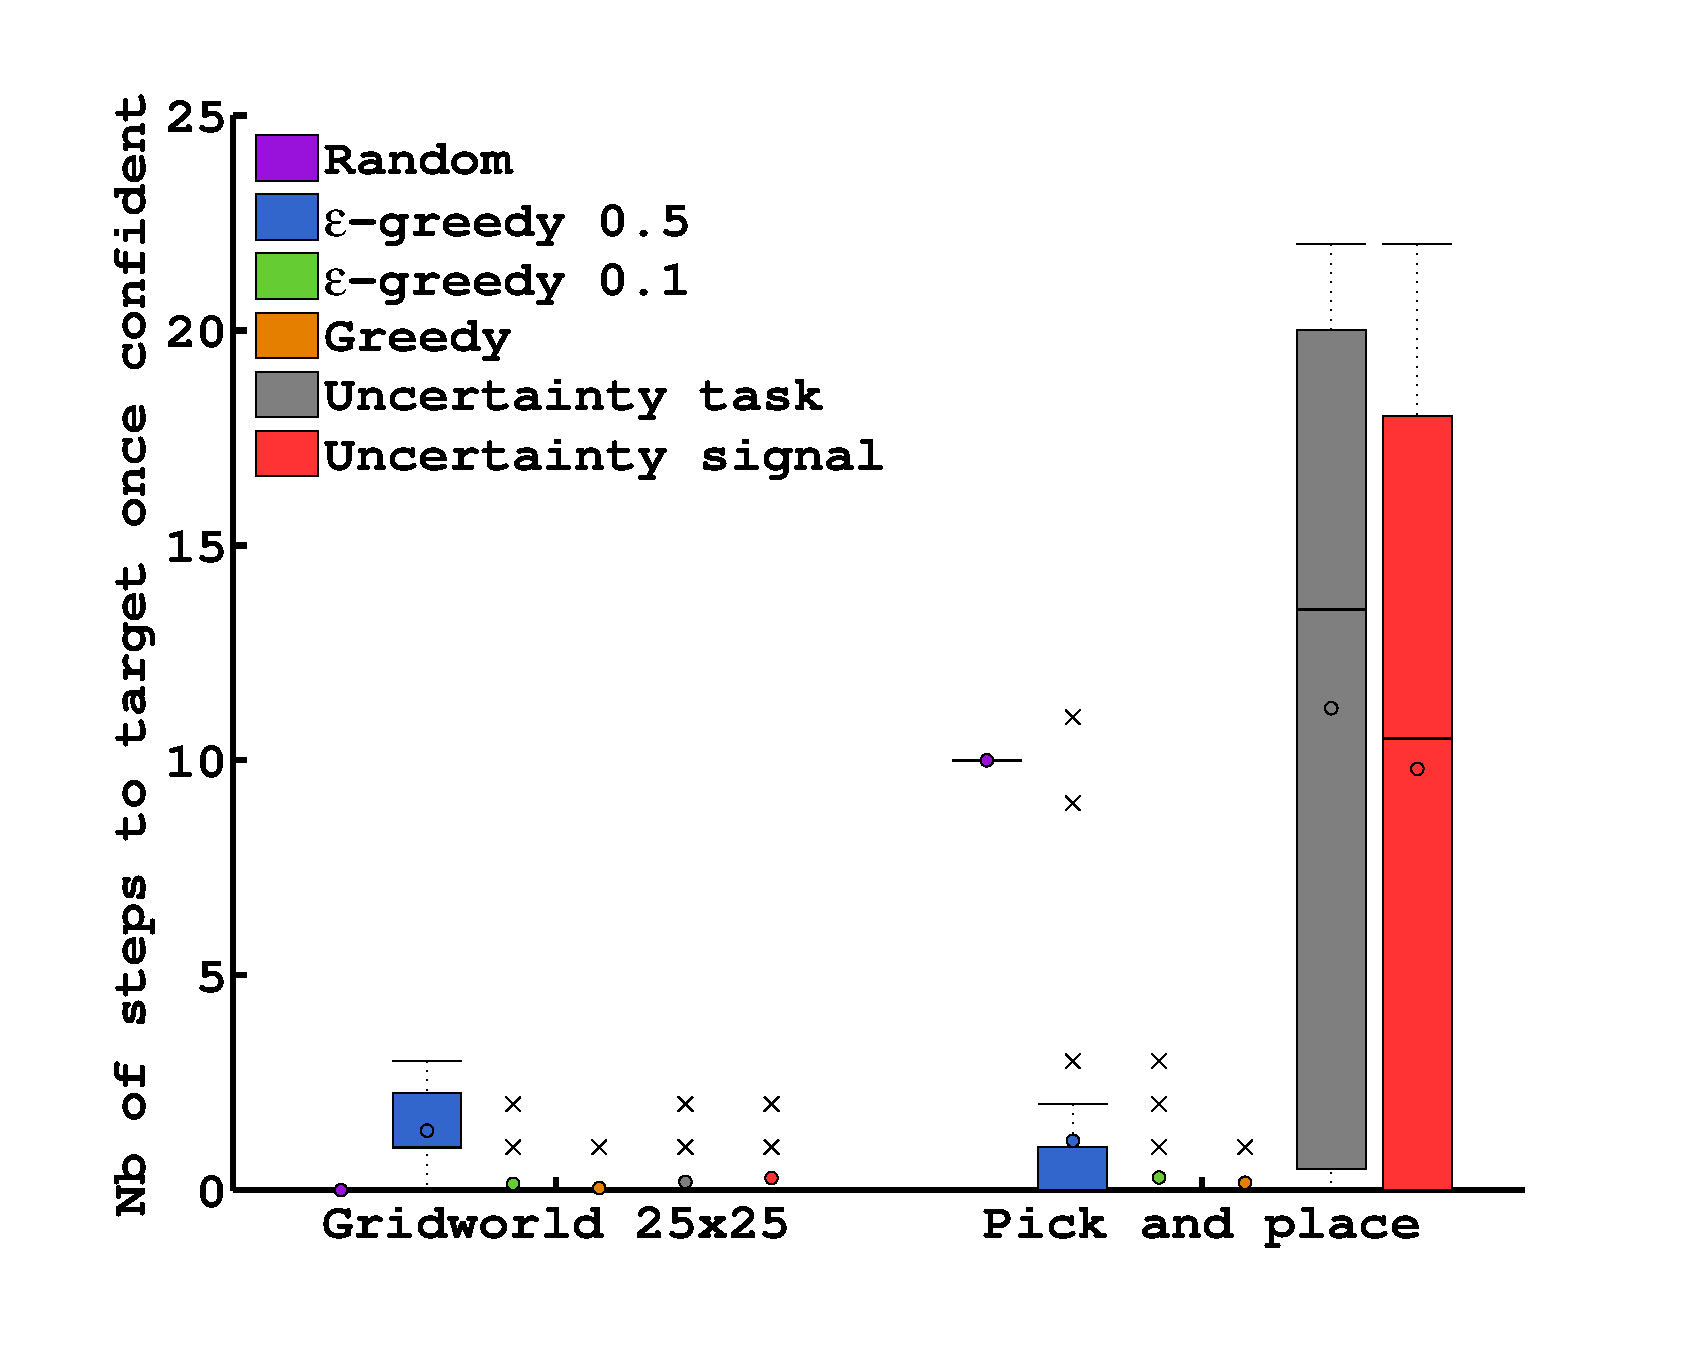
\includegraphics[width=\plotsize\columnwidth]{\imgpath/world_properties/difftargetconfidence.eps}
\caption{Number of action needed to reach the first target when the agent reach confidence level for this target. This plot only consider the runs where a target was reached in less than 100 steps (see Table~\ref{tab:wordlpropertiesnreach}). Random method for the 25x25 grid world is not represented as it never reached any, and random for the pick and place only considers one run.}
\label{fig:wordlpropertiestargetdist}
\end{figure} 

We hypothesized that, given the maze like properties of the pick and place problem, our agent would need to go toward the best hypothesized target states to differentiate between them faster. And therefore that our uncertainty planning method may be more efficient in such case. This hypothesis is not confirmed and requires more investigation on what properties are actually influencing the efficiency of our algorithm and what additional metrics should be considered to improve our strategies. Indeed none of the method presented are considering their performance on the task (yet unknown but estimated) in the action selection process. This is part of the discussion of next subsection.

We note that the Greedy method is going towards the best hypothesis goal state, which confirms our intuition of what is a good planning strategy in such world, but does not explain why our uncertainty method ends-up far from the goal state when the confidence level is reached.
% In order to explain this differences one should analyze the behavior of the agent and the evolution of the probability associated to each task, and check which group of tasks are ruled out first between the Greedy and the uncertainty based method that may explain the differences of behavior observed.

Finally, as for the analysis of the size of the worlds, we note that in chapter~\ref{chapter:planning}~and~\ref{chapter:bci} the greedy method shows very poor performances for 30 dimensional signals. Therefore it is required to compare the performances of the planning methods for a variety of datasets with different dimensionality and quality.

\subsection{Discussion}

The main conclusion of our preliminary study is that we do not understand well the impact of some properties of the world and dataset on the final performance of the system. Many of those properties are tightly linked together and the additional layer of uncertainty inherent to our problem makes the dependencies hard to identifies.

However one important aspect highlighted by the study is that our uncertainty measure should be combined with other metrics to optimize additional criteria on the task. Our measure was developed to discriminate faster the correct hypothesis from the set of possible tasks and not to also execute that task as fast as possible.

We propose two different types of scenario that are likely to be useful in real world scenario: 
\begin{itemize}
\item Target based scenarios: The goal of the agent is to execute one specific action in a particular state and should not make mistakes in the execution of the task. For example, a robot should put one object to the bin for a human. The robot can navigate around of the objects area in order to collect feedback but should only grasp an object and put it to the bin once it is confident about which object to throw away. This includes all the scenario considered in this thesis, and as seen in this section there is room to improve over our uncertainty method by including information about the hypothesized task. A potential avenue is to merge our measure of uncertainty with the optimal policies for each task, such that, for two states with close uncertainty value, the one closer to the target should be preferred. When all task are equally probable, only the uncertainty should be taken into account. And once there is no more uncertainty, i.e. when confidence is reached, the action should be selected according to the task policy. The main problem is about how to weight the two functions.

\item Reward maximization scenarios: In such scenario the goal of the robot is to maximize the reward associated to the correct task. However, many tasks may share some parts of a reward functions. Therefore it is not always necessary to identify the correct task with confidence to collect maximal rewards. For example, in our puddle word scenario of section~\ref{chapter:limitations:continousstate}, two tasks may share the same goal area but different areas to avoid. If the robot can reach the shared goal area by avoiding both negative areas, then the agent will have maximized the collected reward without ever knowing what specific task the user had in mind. Tackling this problem requires a different approach as the agent should now be confident that merging two reward functions is more optimal than trying to differentiate between them. However the robot can not merge all rewards function right from the start as no specific direction will emerge and the correct reward won't be maximized in the long run.
\end{itemize}